\providecommand{\main}{../../..}
\documentclass[\main/main.tex]{subfiles}
\begin{document}

\subsection{Esercizio 5}
Dato un problema di decisione con alternative $X = \{a_1, \ldots , a_5\}$, scenari  $\Omega= {\omega_1, \omega_2}$ e le utilità $u (f (x, \omega))$ riportate nella tabella seguente:

\begin{table}
  \begin{tabular}{|L|L|L|L|L|L|}
    \hline
    u (f (x, \omega)) & a_1 & a_2 & a_3 & a_4 & a_5 \\
    \hline
    \omega_1          & 70  & 90  & 40  & 50  & 20  \\
    \hline
    \omega_2          & 20  & 10  & 30  & 40  & 80  \\
    \hline
  \end{tabular}
\end{table}

\begin{enumerate}[a)]
  \item Si elenchino le eventuali alternative dominate, specificando da quali altre alternative sono dominate.
  \item Si indichi l'alternativa scelta con il criterio del caso pessimo, spiegando il procedimento.
  \item Si indichi l'alternativa scelta con il criterio del rammarico, spiegando il procedimento.
  \item Si mostri come cambia l'alternativa scelta con il criterio di Hurwics al variare del coefficiente di pessimismo $\alpha$.
\end{enumerate}

\subsection{Soluzione esercizio 5}
\subsubsection*{Alternative dominate}
L'alternativa $a_4 \prec a_3$ poiché in entrambi gli scenari le utilità previste sono maggiori. Nei casi alternativi le utilità previste per i due scenari si superano mutualmente, per cui non è possibile identificare nessuna ulteriore coppia di scelte dominata.

\subsubsection*{Criterio del caso pessimo}
Per ogni scelta identifico lo scenario peggiore, quindi tra questi scelgo il migliore. La scelta identificata in questo caso è $a_4$.
\begin{table}
  \begin{tabular}{|L|L|L|L|L|L|}
    \hline
    u (f (x, \omega)) & a_1                   & a_2                   & a_3                   & a_4                    & a_5                    \\
    \hline
    \omega_1          & 70                    & 90                    & 40                    & 50                     & \cellcolor{red!50}  20 \\
    \hline
    \omega_2          & \cellcolor{red!50} 20 & \cellcolor{red!50} 10 & \cellcolor{red!50} 30 & \cellcolor{red!50}  40 & 80                     \\
    \hline
  \end{tabular}
  \caption{In rosso i casi pessimi}
\end{table}

\subsubsection*{Criterio del rammarico}
Vado a calcolare per ogni scelta, per ogni scenario, la distanza dal caso ottimo (detta rammarico). Identifico quindi la distanza massima per ogni scelta e scelgo l'opzione che la minimizza.

\begin{figure}
  \begin{subfigure}{0.49\textwidth}
    \begin{table}
      \begin{tabular}{|L|L|L|L|L|L|}
        \hline
        u (f (x, \omega)) & a_1 & a_2                     & a_3 & a_4 & a_5                    \\
        \hline
        \omega_1          & 70  & \cellcolor{green!50} 90 & 40  & 50  & 20                     \\
        \hline
        \omega_2          & 20  & 10                      & 30  & 40  & \cellcolor{green!50}80 \\
        \hline
      \end{tabular}
      \caption{In verde i casi ottimi}
    \end{table}
  \end{subfigure}
  \begin{subfigure}{0.49\textwidth}
    \begin{table}
      \begin{tabular}{|L|L|L|L|L|L|}
        \hline
        u (f (x, \omega)) & a_1 & a_2 & a_3 & a_4 & a_5 \\
        \hline
        \omega_1          & 20  & 0   & 50  & 40  & 70  \\
        \hline
        \omega_2          & 60  & 70  & 50  & 40  & 0   \\
        \hline
        u_S               & 60  & 70  & 50  & 40  & 70  \\
        \hline
      \end{tabular}
      \caption{Utilità del criterio del rammarico}
    \end{table}
  \end{subfigure}
\end{figure}

La scelta che minimizza il rammarico è la $a_4$.

\subsubsection*{Criterio di Harwics}
Vado a calcolare la combinazione convessa dei due scenari:

\begin{table}
  \begin{tabular}{|L|L|L|L|L|L|}
    \hline
        & a_1                     & a_2                     & a_3                     & a_4                     & a_5                     \\
    \hline
    u_H & 70\alpha + 20(1-\alpha) & 90\alpha + 10(1-\alpha) & 40\alpha + 30(1-\alpha) & 50\alpha + 40(1-\alpha) & 20\alpha + 80(1-\alpha) \\
    \hline
  \end{tabular}
\end{table}

\begin{figure}
  \begin{subfigure}{0.31\textwidth}
    \begin{table}[H]
      \begin{tabular}{|L|L|L|L|L|L|}
        \hline
            & a_1 & a_2 & a_3 & a_4 & a_5 \\
        \hline
        u_H & 70  & 90  & 40  & 50  & 20  \\
        \hline
      \end{tabular}
      \caption{Caso $\pi(\omega_1)=1$: viene scelta $a_2$}
    \end{table}
  \end{subfigure}
  \begin{subfigure}{0.31\textwidth}
    \begin{table}[H]
      \begin{tabular}{|L|L|L|L|L|L|}
        \hline
            & a_1 & a_2 & a_3 & a_4 & a_5 \\
        \hline
        u_H & 20  & 10  & 30  & 40  & 80  \\
        \hline
      \end{tabular}
      \caption{Caso $\pi(\omega_1)=0$: scelta $a_5$}
    \end{table}
  \end{subfigure}
  \begin{subfigure}{0.31\textwidth}
    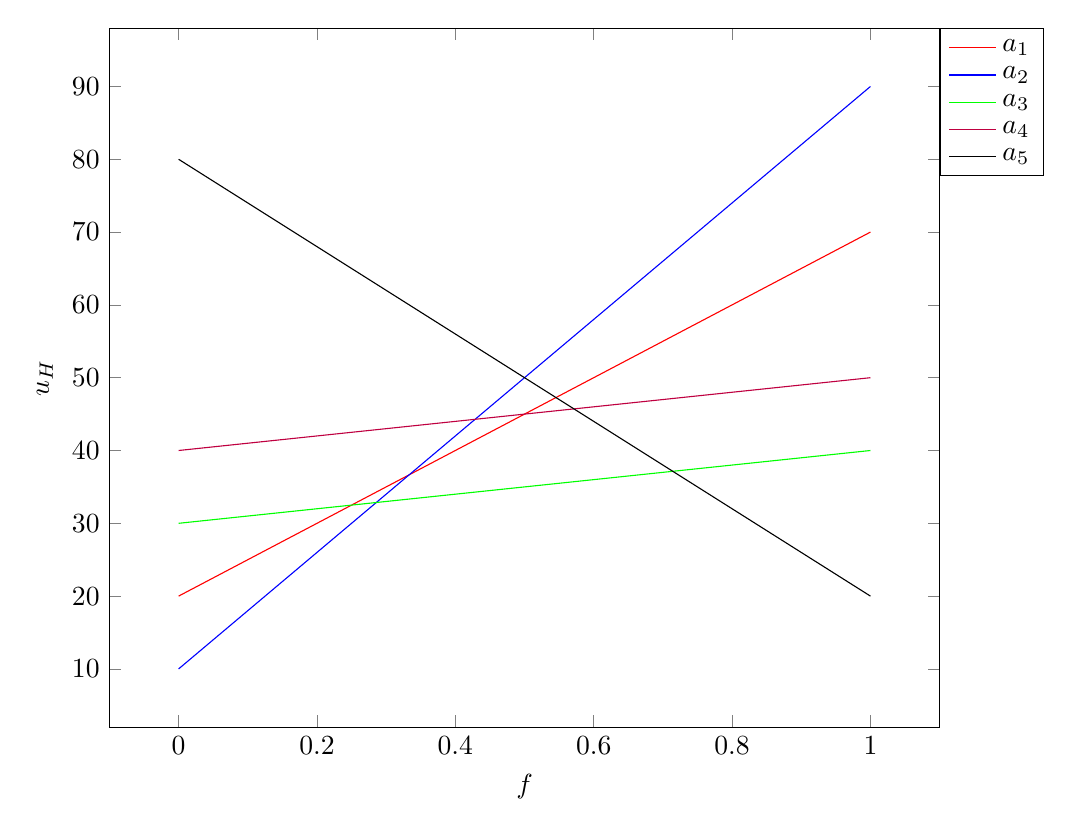
\begin{tikzpicture}
      \begin{axis}[
          width= \textwidth,
          xlabel=$f$,
          ylabel=$u_H$,
          domain=0:1,
          ytick = {0,10,...,90},
          legend style={at={(1,1)},anchor=north west}
        ]
        \addplot[mark=none,color=red]{70*x + 20*(1-x)};
        \addplot[mark=none,color=blue]{90*x + 10*(1-x)};
        \addplot[mark=none,color=green]{40*x + 30*(1-x)};
        \addplot[mark=none,color=purple]{50*x + 40*(1-x)};
        \addplot[mark=none]{20*x + 80*(1-x)};
        \legend{$a_1$,$a_2$,$a_3$,$a_4$,$a_5$}
      \end{axis}
    \end{tikzpicture}
    \caption{L'utilità $u_H$ al variare del coef. di pessimismo $\alpha$}
  \end{subfigure}
\end{figure}

Per $\alpha<0.5$ prevale sempre $a_5$, per $\alpha>0.5$ prevale sempre $a_2$. Questi scenari risultano estremamente sbilanciati.

\end{document}
